\section{Methodology}
\subsection{Datasets and Evaluation}
The in-domain experiment uses the Nickparvar brain tumor MRI collection \cite{nickparvar} with the four categories glioma, meningioma, no tumor, and pituitary tumor. Duplicate and invalid images are removed before the stratified training, validation, and test split; the reported held-out test set contains 1,052 images and is approximately balanced. The configured split proportions are 70/15/15. Images are resized to $224\times224$ and normalized. Training-time transforms include rotation, horizontal reflection, scale changes, intensity variation, and elastic deformation. The primary outcomes are image accuracy and macro F1; specificity and AUC provide complementary class-discrimination summaries. The no-tumor label permits an image-level tumor-presence decision, but no spatial lesion detector is evaluated.

The second experiment uses BraTS 2020 \cite{menze2015,baid2021} to classify high-grade (HGG) versus low-grade (LGG) glioma from axial slices. FLAIR, contrast-enhanced T1, and T2 sequences are stacked as three input channels after per-volume intensity normalization. Tumor-containing axial slices are selected using segmentation masks during dataset construction, with a cap per subject, and are then resized for classification. Grade labels attach to subjects, not independently diagnosed slices. Subjects, rather than slices, are assigned to disjoint stratified splits before slice-level evaluation to avoid within-subject leakage \cite{yagis2021}. The test comparison covers 1,400 slices from 56 subjects, with an approximately 4:1 class imbalance. For patient-level inference, probabilities across a patient's evaluated slices are averaged and the largest mean determines the grade. Mask-based slice selection restricts this study to preselected, tumor-containing slices.

\begin{figure*}[t]
\centering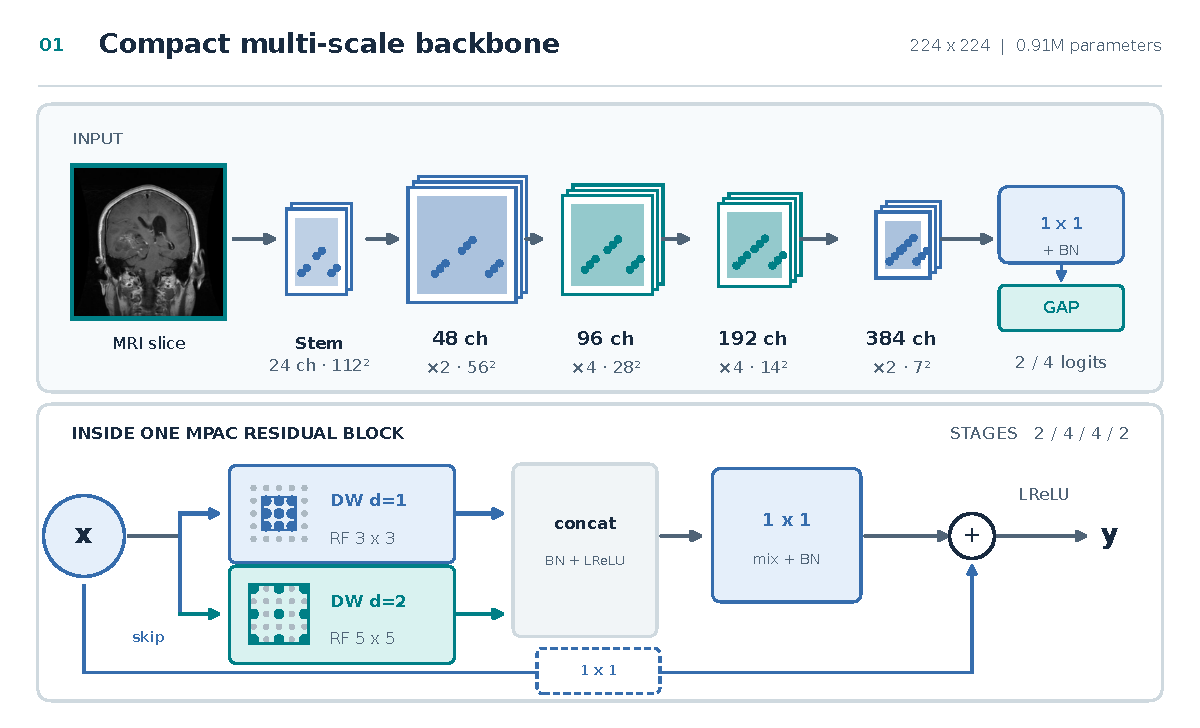
\includegraphics[width=0.88\textwidth]{figures/lsnet_architecture.pdf}
\caption{LS-Net backbone used for both tasks. The stem and four residual MPAC stages reduce spatial resolution while increasing channel width; the task-specific $1\times1$ head maps features to two or four logits. The enlarged block shows the parallel depthwise atrous paths (dilations 1 and 2), channel mixing, and residual connection.}\label{fig:lsnet-architecture}
\end{figure*}

\subsection{Models and Training}
We study fine-tuned ResNet-50, ResNet-18, VGG-16, EfficientNet-B0, and MobileNetV2 alongside compact scratch-trained LS-Net, ResNet-Tiny, MPAC-ResNet-Tiny, EfficientNet-Tiny, and MobileNet-Tiny. The hybrid MPAC-ResNet is included as a separate, above-1M comparison and is not counted as satisfying the strict sub-1M constraint. The compact LS-Net implementation adapts the architecture of Kyrkou \cite{kyrkou2026} with a strided stem and four stages built from residual multi-path atrous blocks (Fig.~\ref{fig:lsnet-architecture}). Each block computes parallel depthwise $3\times3$ convolutions with dilation factors $1$ and $2$, concatenates their outputs, mixes channels with a pointwise convolution, and adds a residual projection when required. The model has 0.91M parameters in both experiments; the different output heads implement the appropriate task labels.

The shared configuration uses $224\times224$ inputs, batch size 32, AdamW with cosine learning-rate scheduling, and validation macro F1 for checkpoint selection. Class weights are enabled for the imbalanced BraTS task. Multi-seed summaries use seeds 42, 123, and 456, except the TTA ablation, which uses the first two. Because pretrained backbones and scratch-trained compact models lack matched initialization, the results establish attainable performance under the specified protocols rather than isolating parameter count as the only causal factor. The four-class table reports sample standard deviations across three seeds, while the two-seed TTA ablation has different dispersion conventions. Pairwise McNemar tests \cite{mcnemar1947} use matched predictions on the 1,052-image four-class test set, with a nominal $0.05$ significance level; failure to reject a difference is not a formal equivalence test.

\subsection{Multi-Scale Consistency-Guided Test-Time Augmentation}
Let $p_0(y\mid x)$ be the LS-Net softmax probability for the unmodified slice $x$, $\hat y_0=\arg\max_y p_0(y\mid x)$, and $c(x)=\max_y p_0(y\mid x)$. A slice passes through the confidence gate when $c(x)<\tau$. Non-gated slices retain $p_0$ without another network call. Gated slices receive deterministic $0.9\times$ and $1.1\times$ scale views (Fig.~\ref{fig:mcg-tta}), yielding $p_-$ and $p_+$. If both scale-view argmax labels equal $\hat y_0$, the returned probability is the mean of the identity and the two scale-view probabilities. Otherwise, the slice escalates to a six-view mean over the identity, both scale views, horizontal flip, and positive and negative rotations. The rotations follow the configured $15^\circ$ augmentation limit. The averaged probability supplies the final slice decision.

Writing $G=\mathbb{1}[c(x)<\tau]$ and $D=\mathbb{1}[\arg\max p_-\ne\hat y_0\ \mathrm{or}\ \arg\max p_+\ne\hat y_0]$, the number of additional model evaluations per slice is $2G+3GD$. The modelled mean latency is therefore $t_0[1+2\Pr(G)+3\Pr(GD)]$, where $t_0$ is the single-forward baseline under the TTA profiling protocol. This formula accounts for conditional network calls but not transformation overhead or end-to-end clinical workflow time. The two probes are informed by the use of multiple dilation scales; neither dilation nor zoom is asserted to be physically equivalent, and the method should be interpreted as an empirical scale-consistency test. Unlike retraining or ensembling independent models, it adds no learned parameters.

\subsection{Efficiency Metrics}
Parameters, floating-point operations per image, model footprint, and batch-one CPU inference time characterize deployment cost. Throughput is the reciprocal of single-image latency under the reported profiling setup. Efficiency was profiled with single-thread PyTorch 2.x inference on an Intel Core CPU using 50 warm-up and 200 timed iterations. Separately, the TTA ablation reports \emph{modelled} latency from a baseline single-forward estimate of 5.60 ms, a different timing series from the 11.30 ms CPU profile. Multiplying the separately profiled LS-Net latency by the TTA relative factor yields an illustrative effective CPU estimate only. We keep the timing series separate throughout.
